\documentclass[border=4pt,12pt]{standalone}
% House style for redrawn exam diagrams (diagram-v4: 0.4pt lines, filled -latex arrows, fine dashes; stipple and hatching drawn as real dots/lines (no PDF/SVG patterns, so they render in every browser and at any scale); transparent background). Every figure \input's this.
\usepackage{amsmath,amssymb}
\usepackage{txfonts}
\usepackage{pdfrender,xcolor}
% \halo{text}: label on shading. The shading stops just around each letter's outline (a thin knock-out that follows the
% glyphs, like the papers' typesetting), never a box. Owner: "I don't want a box around the text".
\newcommand{\halo}[1]{\leavevmode\rlap{\pdfrender{TextRenderingMode=2,LineWidth=2.2pt,LineJoinStyle=1,StrokeColor=white,FillColor=white}#1}#1}
\usepackage{tikz,pgfplots}
\pgfplotsset{compat=1.18}
\usetikzlibrary{arrows.meta,calc,angles,quotes,patterns,patterns.meta,intersections,positioning,decorations.markings,shapes.geometric}
% Stipple and hatching are drawn as actual dots / lines clipped to the region (path picture), NOT as pattern fills:
% SVG <pattern> fills vanish or blur when browsers scale the image, so the owner could not see the shading.
% Each dot is a 0.72pt square (keeps SVGs small; reads as a dot at print size). Dots sit on one global staggered grid, so neighbouring regions line up.
\makeatletter
\newdimen\ex@x \newdimen\ex@y \newdimen\ex@xa \newdimen\ex@ya \newdimen\ex@xb \newdimen\ex@yb \newcount\ex@row
\def\exam@stipplecolor{black!75}\def\exam@dotr{0.42pt}\def\exam@dotgap{2.5}
\def\ex@rowdots{\ifdim\ex@x<\ex@xb \pgfpathrectangle{\pgfqpoint{\dimexpr\ex@x-0.36pt\relax}{\dimexpr\ex@y-0.36pt\relax}}{\pgfqpoint{0.72pt}{0.72pt}}\advance\ex@x by \exam@dotgap pt\relax\expandafter\ex@rowdots\fi}
\def\exam@stipple{%
  \pgftransformreset% dots are sized in real points even inside scaled pictures
  \pgfpointanchor{path picture bounding box}{south west}\ex@xa=\pgf@x \ex@ya=\pgf@y
  \pgfpointanchor{path picture bounding box}{north east}\ex@xb=\pgf@x \ex@yb=\pgf@y
  \pgfsetfillcolor{\exam@stipplecolor}\pgfmathsetmacro\ex@h{\exam@dotgap/2}%
  \pgfmathtruncatemacro\ex@r{floor(\ex@ya/\ex@h)-1}\ex@row=\ex@r\relax
  \ex@y=\ex@r\dimexpr\ex@h pt\relax
  \loop\ifdim\ex@y<\ex@yb
    \pgfmathtruncatemacro\ex@c{floor(\ex@xa/\exam@dotgap)-1}\ex@x=\ex@c\dimexpr\exam@dotgap pt\relax
    \ifodd\ex@row \advance\ex@x by \ex@h pt\fi
    \ex@rowdots
    \advance\ex@y by \ex@h pt \advance\ex@row by 1
    \ifnum\numexpr\ex@row-(\ex@row/4)*4\relax=0 \pgfusepath{fill}\fi% flush every 4 rows: bounded TeX memory, few clip copies in the SVG
  \repeat\pgfusepath{fill}}
\newdimen\ex@d
\def\exam@hatch#1{% #1 = 1 for /, -1 for \ ; lines 45 degrees, 3pt apart
  \pgftransformreset
  \pgfpointanchor{path picture bounding box}{south west}\ex@xa=\pgf@x \ex@ya=\pgf@y
  \pgfpointanchor{path picture bounding box}{north east}\ex@xb=\pgf@x \ex@yb=\pgf@y
  \ex@d=\dimexpr\ex@yb-\ex@ya\relax \ex@x=\dimexpr\ex@xa-\ex@d\relax
  \loop\ifdim\ex@x<\ex@xb
    \ifnum#1>0 \pgfpathmoveto{\pgfqpoint{\ex@x}{\ex@ya}}\pgfpathlineto{\pgfqpoint{\dimexpr\ex@x+\ex@d\relax}{\ex@yb}}%
    \else \pgfpathmoveto{\pgfqpoint{\ex@x}{\ex@yb}}\pgfpathlineto{\pgfqpoint{\dimexpr\ex@x+\ex@d\relax}{\ex@ya}}\fi
    \advance\ex@x by 4.24pt
  \repeat
  \pgfsetlinewidth{0.4pt}\pgfsetstrokecolor{black}\pgfusepath{stroke}}
\def\examstipple{\exam@stipple}\def\examhatch{\exam@hatch}\def\examsetstipplecolor#1{\def\exam@stipplecolor{#1}}\def\examsetdotgap#1{\def\exam@dotgap{#1}}
\makeatother
% (legacy pattern kept for old files)
% staggered stipple like the NESA papers' dotted shading
\pgfdeclarepatternformonly{exam stipple}{\pgfpointorigin}{\pgfqpoint{2.2pt}{2.2pt}}{\pgfqpoint{2.2pt}{2.2pt}}{%
  \pgfpathcircle{\pgfqpoint{0.55pt}{0.55pt}}{0.42pt}\pgfpathcircle{\pgfqpoint{1.65pt}{1.65pt}}{0.42pt}\pgfusepath{fill}}
\tikzset{
  every picture/.style={line width=0.6pt, >={Latex[length=2mm,width=1.3mm]}},
  curve/.style={line width=0.6pt},
  open arrow/.style={-{Latex[length=2mm,width=1.3mm]}},  % owner: filled -latex heads everywhere, no open chevrons
  aux/.style={dash pattern=on 2pt off 1.5pt, line width=0.6pt},
  shade/.code={\def\exA{#1}\def\exB{none}\ifx\exA\exB\else\pgfkeysalso{fill=black!18}\fi},
  shade/.default=on,
  shade dots/.style={fill=none, path picture={\examstipple}},
  stipple color/.code={\examsetstipplecolor{#1}},
  stipple gap/.code={\examsetdotgap{#1}},
  shade dense dots/.style={fill=none, stipple gap=1.6, path picture={\examstipple}},
  shade hatch/.style={fill=none, path picture={\examhatch{1}}},
  shade hatch reverse/.style={fill=none, path picture={\examhatch{-1}}},
  shade solid/.style={fill=black},
  pt/.style={circle, fill, inner sep=1.1pt},
  open pt/.style={circle, draw, fill=white, inner sep=1.1pt},
}
\pgfplotsset{
  exam axes/.style={axis lines=middle, axis line style={->}, xlabel={$x$}, ylabel={$y$},
    xlabel style={anchor=west}, ylabel style={anchor=south}, tick label style={font=\small},
    every axis plot/.append style={line width=0.6pt, black}, samples=200, clip=false,
    enlargelimits=false, axis on top},
}

\begin{document}
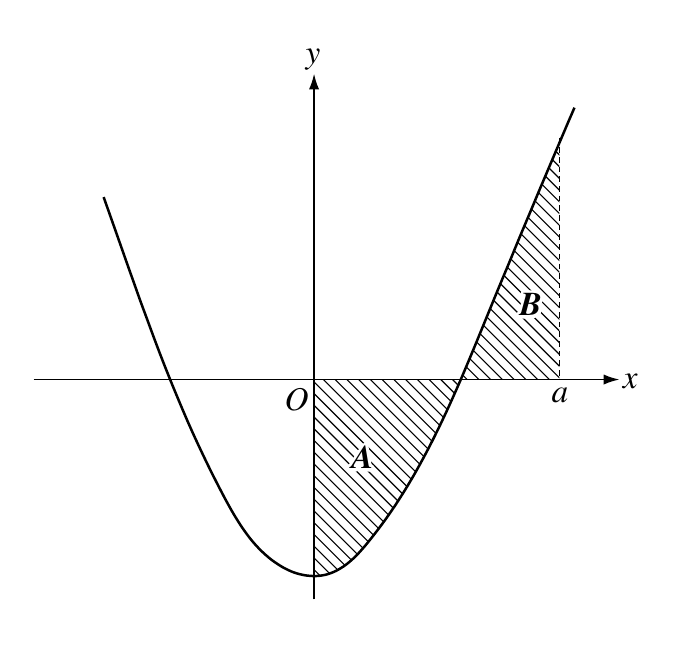
\begin{tikzpicture}[x=0.0127cm, y=-0.0127cm, font=\fontsize{12}{14}\selectfont]
\begin{scope}\clip (287.5,352) rectangle (600,600);
\path[shade hatch reverse] plot[smooth] coordinates {(140,345.5) (143.4,354.4) (146.9,363.2) (150.5,372.1) (154.1,380.8) (157.9,389.5) (161.7,398.3) (165.6,406.9) (169.5,415.5) (173.7,424.2) (177.8,432.7) (182,441.1) (186.3,449.5) (190.7,457.9) (195.2,466.2) (199.8,474.6) (204.5,482.8) (209.1,490.8) (213.8,498.3) (218.6,505.4) (223.7,512) (229.2,518.4) (235,524.4) (241.1,530.1) (247.2,535.1) (253.4,539.3) (259.9,542.7) (266.3,545.3) (272.9,547.1) (279.8,548) (286.9,548.2) (293.8,547.7) (300.6,546.3) (307.1,544.1) (313,541.3) (318.7,537.5) (324.4,532.8) (330.3,527) (336.3,520.6) (342.1,513.9) (347.7,506.9) (353.2,499.7) (358.4,492.3) (363.6,484.7) (368.6,477) (373.5,469.1) (378.4,460.9) (383.1,452.8) (387.7,444.7) (392.2,436.4) (396.7,427.9) (401.1,419.6) (405.4,411.1) (409.7,402.6) (413.8,394.1) (417.9,385.4) (422,376.8) (426,368.1) (430,359.4) (434,350.5)} -- cycle;
\end{scope}
\begin{scope}\clip (0,0) rectangle (532,352);
\path[shade hatch reverse] plot[smooth] coordinates {(429,361.5) (430.8,357.2) (432.6,353) (434.4,348.7) (436.2,344.5) (438,340.2) (439.8,336) (441.6,331.7) (443.4,327.5) (445.2,323.2) (447,318.9) (448.8,314.7) (450.5,310.5) (452.3,306.2) (454.1,301.9) (455.9,297.7) (457.7,293.4) (459.5,289.2) (461.3,284.9) (463.1,280.7) (464.8,276.4) (466.6,272.1) (468.4,267.9) (470.2,263.7) (472,259.4) (473.7,255.1) (475.5,250.9) (477.3,246.6) (479,242.4) (480.8,238.1) (482.6,233.9) (484.3,229.6) (486.1,225.3) (487.9,221) (489.6,216.8) (491.4,212.5) (493.1,208.3) (494.9,204) (496.7,199.7) (498.4,195.5) (500.1,191.2) (501.9,186.9) (503.6,182.7) (505.4,178.4) (507.1,174.1) (508.9,169.8) (510.6,165.6) (512.3,161.3) (514.1,157) (515.8,152.8) (517.5,148.5) (519.3,144.2) (521,139.9) (522.7,135.7) (524.4,131.4) (526.1,127.1) (527.8,122.9) (529.6,118.6) (531.3,114.3) (533,110)} -- (532,110) -- (532,400) -- cycle;
\end{scope}
\draw[->] (6,352) -- (592,352);
\draw[->] (286.5,572) -- (286.5,46);
\draw[aux] (532,110) -- (532,352);
\draw[line width=0.9pt] plot[smooth] coordinates {(76,169.5) (82.19,187) (88.33,204.4) (94.38,221.6) (100.5,239) (106.7,256.4) (112.8,273.6) (119.2,290.9) (125.5,308) (131.9,325) (138.4,341.7) (145.2,358.6) (152.1,375.2) (159.1,391.7) (166.4,408.1) (174,424.4) (181.7,440.4) (189.7,456.3) (198,472.2) (206.2,486.8) (214.8,500.4) (223.9,512.7) (233.5,523.2) (243.9,532.3) (255.2,539.8) (266.1,544.9) (277.2,547.8) (288.2,548.6) (298.4,547.2) (308.3,543.5) (318.2,537.4) (328,528.9) (338.1,517.7) (348.6,504.5) (358.7,490.9) (368.5,476.6) (377.8,462) (386.6,447.2) (395.1,431.9) (403.3,416.3) (411.2,400.4) (418.8,384.4) (426.2,368.1) (433.4,351.7) (440.5,334.9) (447.5,318.1) (454.5,301) (461.5,283.9) (468.4,267) (475.5,249.9) (482.6,232.9) (489.6,215.8) (496.7,198.8) (503.8,182) (510.9,164.9) (518.1,147.9) (525.3,130.9) (532.5,113.9) (539.7,96.95) (547,80)};
\node at (285.5,32) {$y$};
\node at (602,354) {$x$};
\node at (532.5,368) {$a$};
\node at (269,372) {$O$};
\node at (333.5,430) {\halo{$\boldsymbol{A}$}};
\node at (502.5,277) {\halo{$\boldsymbol{B}$}};
\end{tikzpicture}
\end{document}
